\chapter{Background}

\section{Automatic Drum Transcription}

As mentioned, \gls{ADT} describes the task of transcribing symbolic notation for drums from audio. To be even more descriptive, \gls{ADT} can be split into further tasks. From least to most complex we have: \gls{DSC}, where we classify drum instruments from isolated recordings. \gls{DTD}, where we transcribe audio containing exclusively drum instruments. \gls{DTP}, where we transcribe audio containing drum instruments, and additional percussive instruments which the transcription should exclude. Finally, we have \gls{DTM}, which describes the task of drum transcription with audio containing both drum, and melodic instruments.~\cite{8350302}

In this thesis, we will focus on the most complex of these, namely \gls{DTM}. Intuitively, we want to develop a deep learning model which, given input audio, has the ability to detect and classify different drum instrument onsets (events), while selectively ignoring unrelated, melodic instruments.

This task comes with difficulties not seen in the less complex tasks. Zehren et al.~\cite{signals4040042} describes one example, in where \textit{"melodic and percussive instruments can overlap and mask eachother..., or have similar sounds, thus creating confusion between instruments"}.

Deep learning has shown to be a promising method to solve such a task, and several different approaches have been tried, many with great success. Vogl et al.~\cite{vogl2018multiinstrumentdrumtranscription, Vogl2017DrumTV} displayed good results with both a convolutional, and a convolutional-recurrent neural network. Zehren et al.~\cite{signals4040042, zehren2024analyzingreducingsynthetictorealtransfer} focused on datasets, showing that the amount of data and quality of data are equally important to get good performance. Most recently, Chang et al.~\cite{chang2024yourmt3multiinstrumentmusictranscription} explored an autoregressive, language model approach. This approach explored multi-instrument transcriptions, but their results on \gls{ADT} were notable.

This reinforces the fact that there still exist many approaches to attempt, which could lead to a general improvement on \gls{ADT} models.

\section{Audio}

Sound has be described as \textit{"the sensation caused in the nervous system by vibration of the delicate membranes of the ear."}~\cite{1953fundamentals}. In short, sound is the human perception of acoustic waves in a transition medium, like air. These waves, consisting of vibrating molecules, get sensed by our auditory organs and perceived by the brain. 

Thus sound can be described as the propogation and perception of waves. Mathematically, waves can be studied as signals~\cite{8454362}. To represent these sounds digitally, as \textit{audio}, one can express these waves as a signal, giving rise to the \textit{waveform}. The waveform is a representation of a signal as a graph, and charts the amplitude, or strength of the signal, over time.

\begin{figure}[H]
    \centering
    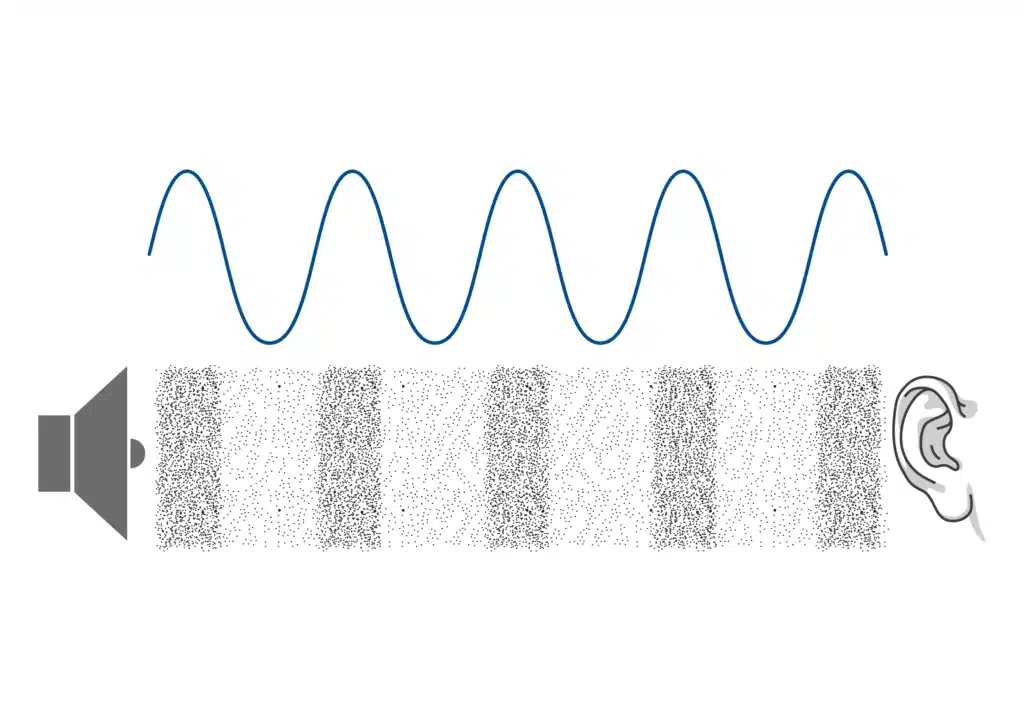
\includegraphics[scale=0.3]{figures/waveform}
    \caption{Soundwave to waveform relationship}
    \label{WaveformFigure}
\end{figure}

For monophonic sound, this waveform is a one-dimensional representation. Even though this is an excellent way of storing audio digitally, it is very compact. There have been deep learning models working directly with these waveforms, e.g. Oord et al.'s WaveNet~\cite{oord2016wavenetgenerativemodelraw}, however the task of parsing and perceiving such a signal is a complex one.

\subsection{Fourier Transform}

The Fourier Transform is a mathematical transformation which, given a frequency, computes its significance, or intensity, in a given signal. As we've established, audio is represented as a signal, and we can therefore use this transform to turn this audio signal into frequency space. 

The fourier transform is a complex transformation, but we can attempt an intuitive explanation. Trigonometric functions have the property that they are \textit{orthogonal} to eachother if they have different integer frequencies. In laymen's terms, the \textit{area under the curve} of the product between to sines (or cosines) are zero if they have a different frequency.

$$ \int_{\infty}^{\infty} \text{sin}(ax) \text{sin}(bx) dx = 0, \ a \neq b \wedge (a, b) \in \mathbb{Z} $$

\textcolor{red}{Continue explanation but maybe not as mathy? Define and explain the core Fourier transform equation.}

By doing such a transform, we turn our temporal data into spectral data. This initively \textit{untangles} our signal into its respective base frequencies. Such an transformation could lessen the complexity of the task, making \textit{understanding} of audio easier.

\begin{figure}[H]
    \centering
    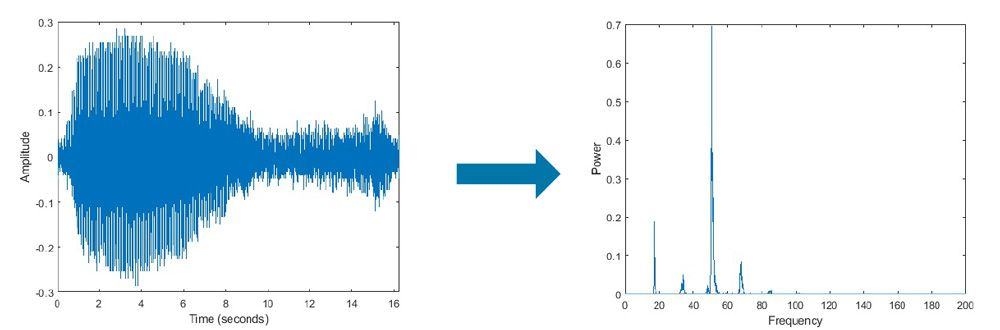
\includegraphics[scale=0.4]{figures/fft.jpg}
    \caption{Application of a Fourier Transform}
    \label{FTFigure}
\end{figure}

The information obtained from the Fourier Transform is \textit{complex}. This means every value consists of a \textit{real} part and an \textit{imaginary} part. The real part consists of the amplitude of a certain frequency, where as the imaginary part consists of the phase.

\subsection{Discrete Fourier Transform}

The Fourier Transform is defined as an integral over continuous time. On computers, instead of storing signals continuously we store signals using a discrete number of samples. Each signal's \textit{sampling rate} describes how many samples a signal contains per second of audio, and is denoted in \textit{Hz}.

To extract frequency values from these signals, we instead have to use the \gls{DFT}. Intuitively this works as the normal Fourier Transform, but ported to work on discrete-valued signals. It is given by the formula $$ X_k = \sum^{N - 1}_{n=0}{x_n \cdot e^{-i 2\pi \frac{k}{N} n}} $$, where $k$ denotes the frequency and $N$ the number of discrete samples.

\subsection{Nyquist frequency}

When we discretize a signal, e.g. when going from continuous audio waves in the air to discrete audio signals on a computer, we could lose some information. T discrete representation of the signal is an \textit{approximation}, which quality is directly dependent on the sampling rate. The higher the sampling rate, the \textit{closer} we are the original, continuous signal. However a higher sampling rate comes at the cost of needing to store these signals at a higher precision. A lower sampling rate would need less information stored, but this also mean a less precise signal approxmation.

\textit{Aliasing} is the phenomena where new frequencies seem to emerge in undersampled signals. For a given discrete signal, the \textit{Nyquist frequency}, equal to half the sampling rate, is the maximum frequency a signal accurately can represent. Thus to prevent aliasing, one would need to store a signal with a sampling rate of at least double the maximum frequency.

\begin{figure}[H]
    \centering
    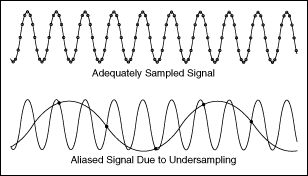
\includegraphics[scale=2.0]{figures/signalaliasing.png}
    \caption{Example of aliasing in an undersampled signal.}
    \label{AliasingFigure}
\end{figure}

Regarding the \gls{DFT}, it here directly follows that the maximum frequency we accurately could extract information about is proportional to the sampling rate of the signal.

\subsection{Fast Fourier Transform}

Keen-eyed computer scientists may have spotted that the \gls{DFT} runs in $\mathcal{O}(n^2)$ time as we, for every frequency in the range $[0, N]$ have to sum over $N$ different values. In other words, the \gls{DFT} algorithm scales quite poorly. Take into account that the standard sampling rate for audio is $44.1 \text{kHz}$, i.e. $44100 \text{Hz}$, then we can see that the \gls{DFT} could be inefficient.~\cite{pras2010sampling}

The \gls{FFT} is an algorithm which solves this problem, and instead computes the \gls{DFT} of a signal within $\mathcal{O}(n\log{n})$ time. Described by Gilbert Strang as \textit{"the most important numerical algorithm of our lifetime"}~\cite{strang1993wavelettransformsversusfourier}, this practically solves our scaling problem, and allows us to efficiently extract spectral information from a signal regardless of sampling rate.

There exist many different implementations of the \gls{FFT}. However the Cooley-Tukey algorithm is by far the most used \gls{FFT} and optimizes calculations through a \textit{divide and conquer} approach, utilizing previous calculations to compute others.~\cite{d3ea2d52-5ab2-3128-8b80-efb85267295d}

\subsection{Short-time Fourier Transform}

The Fourier Transform comes with some drawbacks, notably how by moving from time space into frequency space, we lose temporal information. For certain tasks this might be sufficient, but the temporal dimension is vital when working with transcriptions and \gls{ADT} tasks. We've seen how the Fourier Transform computes the frequencies of a signal, but what happens if we had applied the same transform to smaller, \textit{partitions} of a signal.

This leads us to the \gls{STFT}. By instead of transforming the whole signal, we transform smaller \textit{windows}, we could gain insight into the frequency space while keeping temporal information relatively intact. This turns our data from being one-dimensional into two-dimensional, giving us insight into the intensities of different frequencies, along different timesteps.

\textcolor{red}{Talk more about the partitioning. The window functions applied, and why. Spectral leakage..}

\begin{figure}[H]
    \centering
    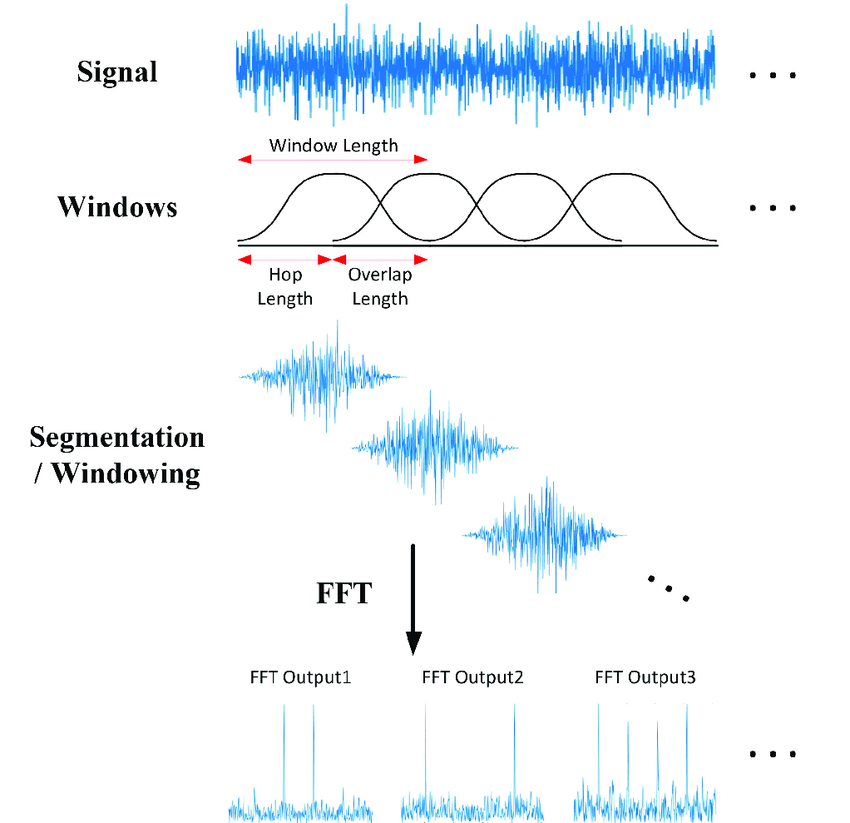
\includegraphics[scale=0.35]{figures/stft}
    \caption{Example of the \gls{STFT}}
    \label{STFTFigure}
\end{figure}

\subsection{Spectrogram}

The \gls{STFT}, as the standard Fourier Transform, returns the data as complex values. To turn these into strictly real values without discarding data, we could compute the spectrogram. This is done by squaring the absolute value of each complex number. 

\begin{figure}[H]
    \centering
    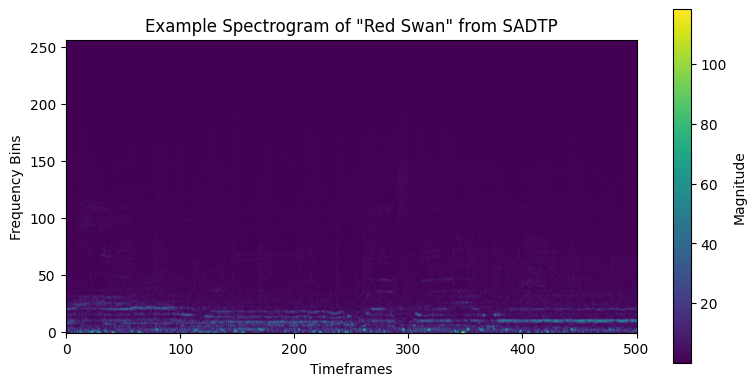
\includegraphics[scale=0.35]{figures/spectrogram}
    \caption{The spectrogram of an audio signal}
    \label{SpectrogramFigure}
\end{figure}

\textcolor{red}{Mention something about how we are losing some, or all phase information.}

\subsection{Filters}

\textcolor{red}{Explain about spectrogram filtering and filterbanks. Mention mel-filters, logarithmic-filters, and their usages in ADT.}

\subsubsection{Mel Spectrograms}

\subsubsection{Logarithmic Filters}

\section{Transcription}

\textcolor{red}{Explain what a transcription is, and what formats they usually are on. Explain what our model is predicting.}

\subsection{Sheet Music}

\subsection{MIDI Annotations}

\subsection{Activation Functions}

\textcolor{red}{Not the usual "Activation Functions" talked about in Deep Learning, but rather the output of the models. The \textit{confidence} of a class' activation. "Probability of happening".}

\section{Performance Measure}

\textcolor{red}{Mention the different performance measures we have, what they are good for, and which ones are suitable here.}

\textcolor{red}{Also mention what is deemed a "correct prediction", and why we can allow a certain timeframe of "correctness".}